\documentclass[mathserif,spanish]{beamer}

\mode<presentation> {
\usetheme{Warsaw}
\setbeamertemplate{footline}[page number]
}

\usepackage{graphicx}
\usepackage{booktabs} 
\usefonttheme{professionalfonts}
\usepackage{beamerthemesplit}
\usepackage[justification=centering]{caption}
\setbeamertemplate{caption}[numbered]
\usepackage{ragged2e}
\justifying
\usepackage{hyperref}
\usepackage{chngcntr}
\usepackage[utf8]{inputenc} 
\usepackage[spanish]{babel}
\usepackage{listings}
\usepackage{tcolorbox}

% Adjust font size for code
\lstset{
  basicstyle=\ttfamily\large, % increase font size here
  breaklines=true,
  frame=single
}

\title[Modulador y Demodulador FM]{Modelado de un Sistema de Comunicaciones FM}
\subtitle{Equipo B} 
\author[F. Chacón \and G. Araya]{F. Chacón \and G. Arya} 
\institute[Instituto Tecnológico de Costa Rica]{
Instituto Tecnológico de Costa Rica\\
Escuela de Ingeniería Electrónica \\
Nombre del curso: Comunicaciones Eléctricas I\\
Código: EL 5513\\
Profesor: Ing. Leonardo Sandoval Cascante
}
\date{\today}

\begin{document}

\begin{frame}[plain]
    \titlepage
\end{frame}

\begin{frame}{Contenidos}
    \tableofcontents 
\end{frame}

\section{Introducción}

\subsection{Resumen}
\begin{frame}{Resumen}
    \begin{itemize}
        \item Diseño y modelado de un sistema de comunicaciones FM que incluye un modulador y demodulador.
        \item Multiplexación por división de frecuencia de tres señales de audio.
        \item Implementación y simulación en MATLAB/Octave.
    \end{itemize}
\end{frame}

\subsection{Objetivo General}
\begin{frame}{Objetivo General}
    \begin{itemize}
        \item Modelar y simular un sistema de comunicaciones FM utilizando herramientas EDA, reforzando habilidades de trabajo en equipo y técnicas de resolución de problemas.
    \end{itemize}
\end{frame}

\subsection{Objetivos Específicos}
\begin{frame}{Objetivos Específicos}
    \begin{itemize}
        \item Modelar un modulador FM.
        \item Modelar un multiplexor por división de frecuencia.
        \item Modelar un receptor superheterodino.
        \item Modelar un demodulador FM.
        \item Proponer la implementación de circuitos moduladores mediante un simulador.
    \end{itemize}
\end{frame}

\section{Modelado del Sistema}

\subsection{Modelado del Modulador FM}
\begin{frame}{Modelado del Modulador FM}
    \begin{itemize}
        \item Generación de señales de audio independientes.
        \item Multiplexación en frecuencia utilizando subportadoras.
        \item Modulación en frecuencia utilizando una portadora de 110 MHz.
        \item Inclusión de una señal piloto para referencia.
    \end{itemize}
    
\end{frame}

\begin{frame}{Modelado del Modulador FM}
   
    \begin{figure}[h]
        \centering
        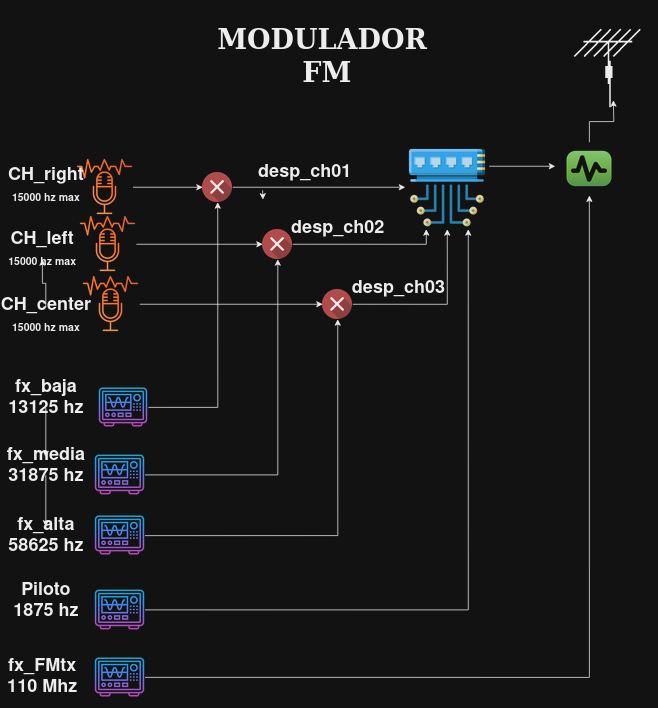
\includegraphics[scale=0.3]{modu1.png}
        \caption{Diagrama del Modulador FM}
    \end{figure}
\end{frame}





\subsection{Modelado del Demodulador FM}
\begin{frame}{Modelado del Demodulador FM}
    \begin{itemize}
        \item Recepción de la señal modulada y mezcla con un oscilador local.
        \item Generación de la señal de frecuencia intermedia (IF) centrada en 10.7 MHz.
        \item Demodulación de las subportadoras para recuperar las señales de audio.
        \item Aplicación de filtros de deénfasis y ajuste de ganancia.
    \end{itemize}
    
\end{frame}

\begin{frame}{Modelado del Demodulador FM}
   
    \begin{figure}[h]
        \centering
        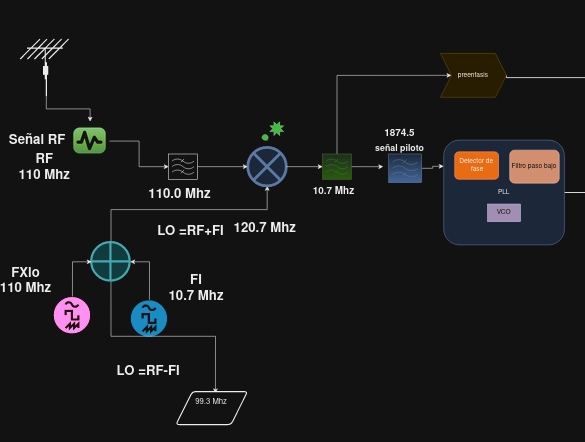
\includegraphics[scale=0.3]{demo_02.png}
        \caption{Diagrama del Demodulador FM parte 1}
    \end{figure}
\end{frame}


\begin{frame}{Modelado del Demodulador FM}
   
    \begin{figure}[h]
        \centering
        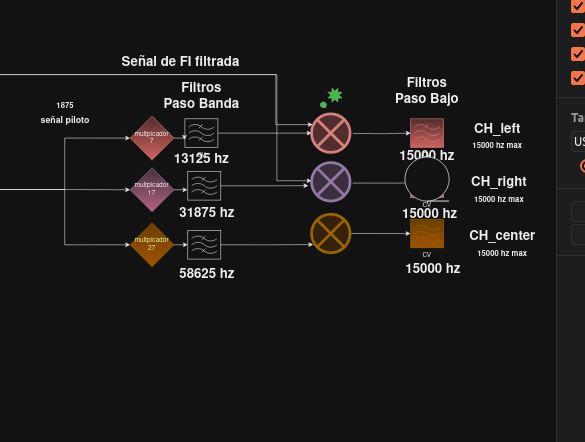
\includegraphics[scale=0.3]{demo_01.png}
        \caption{Diagrama del Demodulador FM parte 2}
    \end{figure}
\end{frame}









\subsection{Distribución de Frecuencias}
\begin{frame}{Distribución de Frecuencias}
    \begin{itemize}
        \item Frecuencia de la portadora: 110 MHz.
        \item Señal piloto: 1875 Hz.
        \item Subportadoras: 13125 Hz, 31875 Hz, 50625 Hz.
        \item Ancho de banda total: 120 kHz.
    \end{itemize}
    \begin{figure}[h]
        \centering
        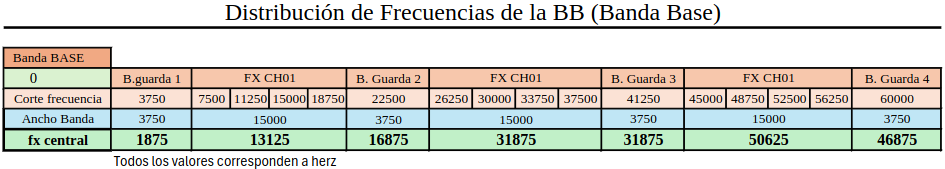
\includegraphics[width=\textwidth]{fx_BB.png}
        \caption{Distribución de Frecuencias en el Sistema}
    \end{figure}
\end{frame}

\section{Implementación del Modulador FM}

\subsection{Parámetros Iniciales del Modulador FM}
\begin{frame}{Parámetros Iniciales del Modulador FM}
    \begin{itemize}
        \item Duración de la señal: 1 segundo.
        \item Frecuencia de muestreo: 25 MHz.
        \item Creación de un vector de tiempo lineal para la duración de la señal.
    \end{itemize}
    \begin{figure}[h]
        \centering
        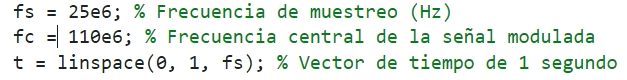
\includegraphics[width=\textwidth]{F_muestreo.png}
        \caption{Código Definición Frecuencia de Muestreo}
    \end{figure}
\end{frame}

\subsection{Generación de Señales y Subportadoras}
\begin{frame}{Generación de Señales y Subportadoras}
    \begin{itemize}
        \item Generación de señales sinusoidales para representar las señales de audio independientes.
        \item Generación de señales sinusoidales para representar las subportadoras.
    \end{itemize}
    \begin{tcolorbox}[colback=yellow!5!white, colframe=yellow!75!black, title=Generación de Señales y Subportadoras, fonttitle=\normalsize, fontupper=\normalsize]
\begin{lstlisting}
% Generación de las señales
fxRight = sin(2*pi*Right*t);
fxLeft = sin(2*pi*Left*t);
fxCenter = sin(2*pi*Center*t);

% Generación de subportadoras
fxPiloto = sin(2*pi*fxpiloto*t);
fxBaja = sin(2*pi*fxbaja*t);
fxMedia = sin(2*pi*fxmedia*t);
fxAlta = sin(2*pi*fxalta*t);
\end{lstlisting}
    \end{tcolorbox}
\end{frame}


\begin{frame}{Generación de Señales y Subportadoras}
    \begin{figure}[h]
        \centering
        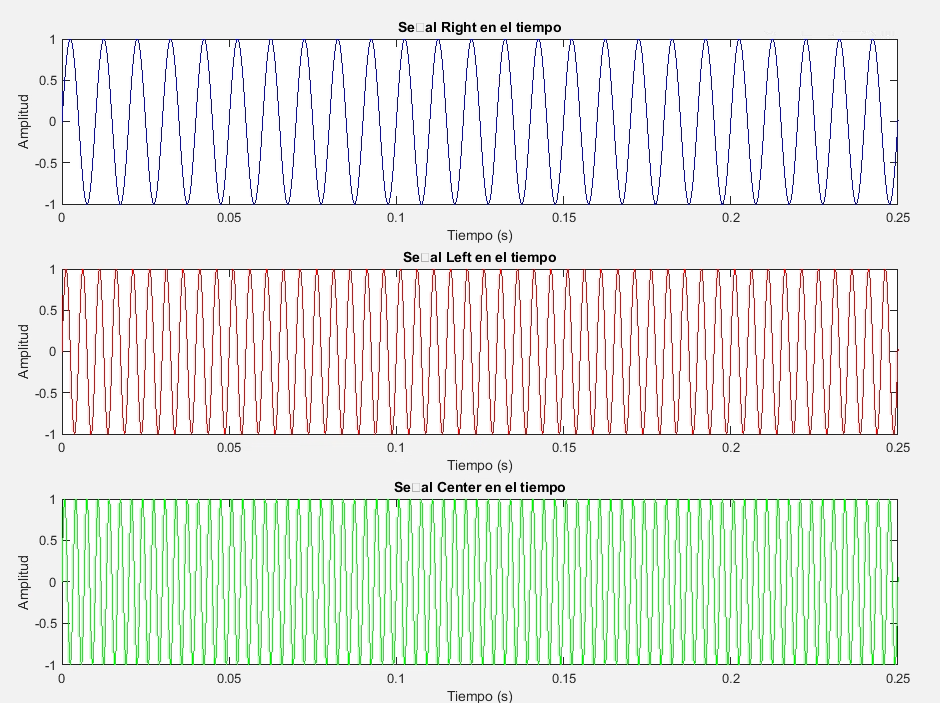
\includegraphics[scale=0.2]{d_tie_CHs.png}
      
        \caption{Señales de los Canales en función del tiempo}
    \end{figure}
\end{frame}

\begin{frame}{Generación de Señales y Subportadoras}
    \begin{figure}[h]
        \centering
        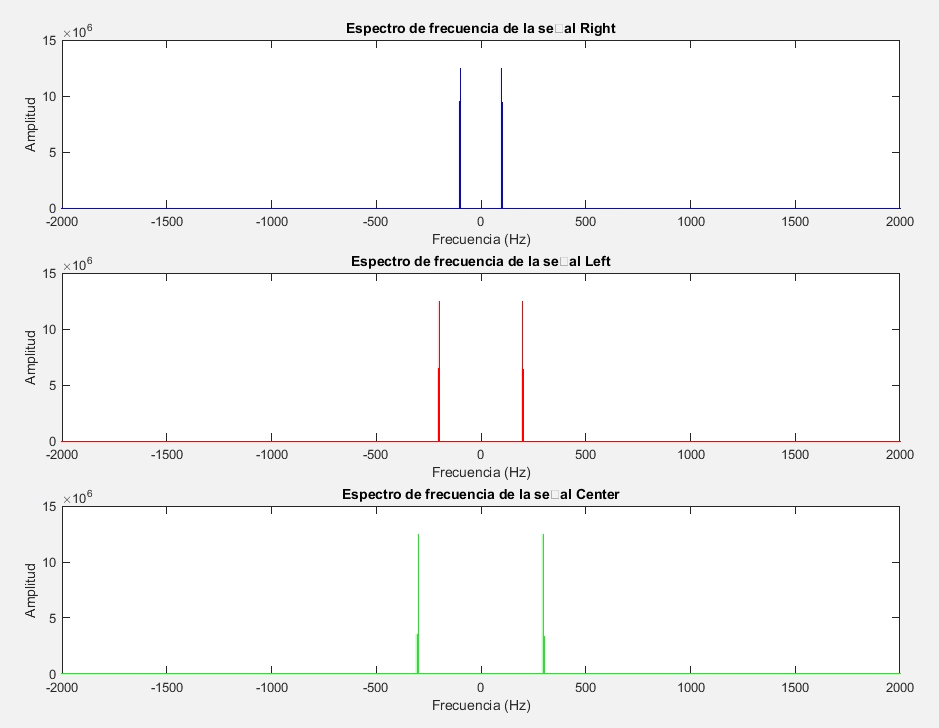
\includegraphics[scale=0.2]{d_fre_CHs.png}
      
        \caption{Señales de los Canales en función de la Frecuencia}
    \end{figure}
\end{frame}

\begin{frame}{Generación de Señales y Subportadoras}
    \begin{figure}[h]
        \centering
        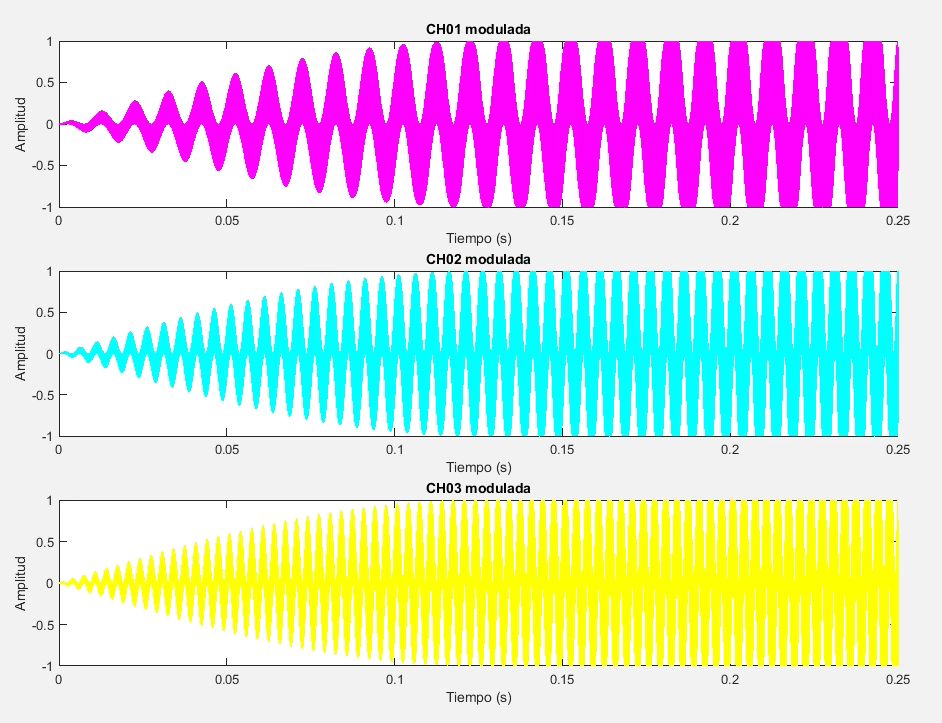
\includegraphics[scale=0.2]{CHs_Modu_Frec.png}
      
        \caption{Canales Modulados en función del tiempo}
    \end{figure}
\end{frame}

\begin{frame}{Generación de Señales y Subportadoras}
    \begin{figure}[h]
        \centering
        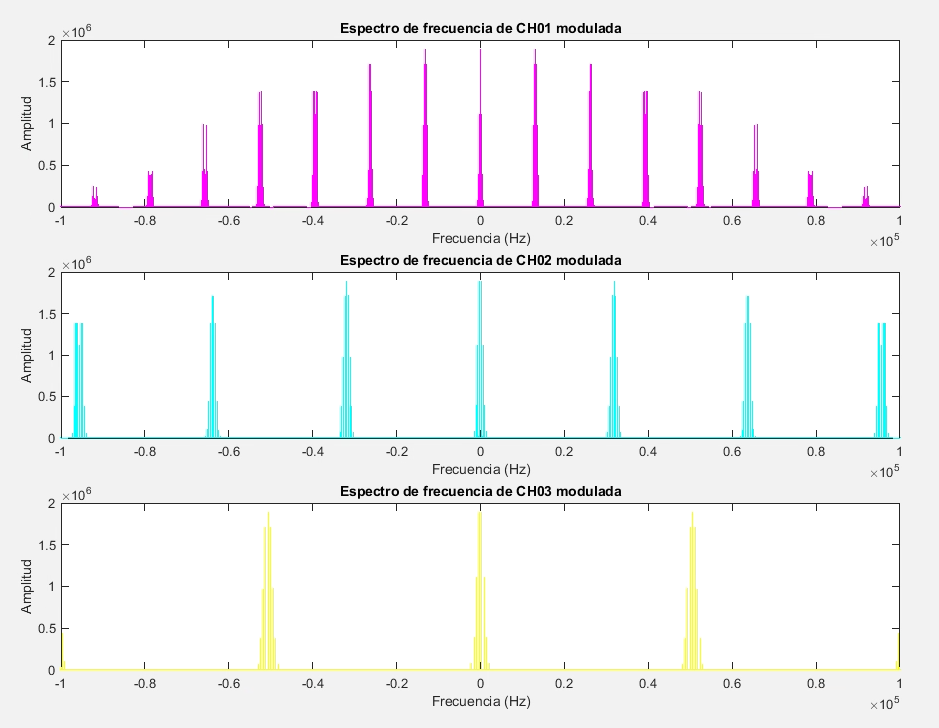
\includegraphics[scale=0.2]{CHs_mod_Tiem.png}
      
        \caption{Canales Modulados en función de la Frecuencia}
    \end{figure}
\end{frame}






\subsection{Preénfasis y Multiplexación}
\begin{frame}{Preénfasis y Multiplexación}
    \begin{itemize}
        \item Aplicación de un filtro de preénfasis para amplificar las altas frecuencias.
        \item Desplazamiento de señales en frecuencia y combinación con la señal piloto.
    \end{itemize}
    \begin{tcolorbox}[colback=yellow!5!white, colframe=yellow!75!black, title=Preénfasis y Multiplexación, fonttitle=\normalsize, fontupper=\normalsize]
\begin{lstlisting}
% Implementar preénfasis (filtrado FIR)
preemphasis = [1 -0.95];
fxRight_preemphasis = filter(preemphasis, 1, fxRight);
fxLeft_preemphasis = filter(preemphasis, 1, fxLeft);
fxCenter_preemphasis = filter(preemphasis, 1, fxCenter);

% Desplazamiento por medio de multiplicación 
desCH01 = sin(2*pi*(fxRight_preemphasis + fxBaja).*t);
desCH02 = sin(2*pi*(fxLeft_preemphasis + fxMedia).*t);
desCH03 = sin(2*pi*(fxCenter_preemphasis + fxAlta).*t);

% Multiplexación de las subportadoras de audio con la frecuencia piloto
subporta = fxPiloto + desCH01 + desCH02 + desCH03;
\end{lstlisting}
    \end{tcolorbox}
\end{frame}

\subsection{Modulación FM}
\begin{frame}{Modulación FM}
    \begin{itemize}
        \item Modulación de la señal multiplexada utilizando una portadora de 110 MHz.
        \item Almacenamiento de la señal modulada y variables necesarias para su posterior uso en la demodulación.
    \end{itemize}
    \begin{tcolorbox}[colback=yellow!5!white, colframe=yellow!75!black, title=Modulación FM, fonttitle=\normalsize, fontupper=\normalsize]
\begin{lstlisting}
% Modulación FM
FMmodulada = cos(2*pi*FXporta*t + IndMod*subporta);

% Guardar la señal modulada y variables necesarias en un archivo
save('FMmodulada.mat', 'FMmodulada', 'fs', 'FXporta', 'IndMod', 'subporta');
\end{lstlisting}
    \end{tcolorbox}
\end{frame}

\subsection{Visualización en el Dominio de la Frecuencia}
\begin{frame}{Visualización en el Dominio de la Frecuencia}
    \begin{itemize}
        \item Cálculo de la transformada de Fourier para analizar las señales en el dominio de la frecuencia.
        \item Creación de gráficos para visualizar las señales en el dominio del tiempo y de la frecuencia.
    \end{itemize}
    \begin{tcolorbox}[colback=yellow!5!white, colframe=yellow!75!black, title=Visualización en el Dominio del Tiempo y Frecuencia, fonttitle=\normalsize, fontupper=\normalsize]
\begin{lstlisting}
% Transformada de Fourier
N = length(t);
f = (-fs/2 : fs/N : fs/2 - fs/N); % Vector de frecuencias

% Cálculo de la FFT para cada señal y operación
FFT_fxRight = fftshift(fft(fxRight, N));
FFT_fxLeft = fftshift(fft(fxLeft, N));
FFT_fxCenter = fftshift(fft(fxCenter, N));
FFT_modCH01 = fftshift(fft(desCH01, N));
FFT_modCH02 = fftshift(fft(desCH02, N));
FFT_modCH03 = fftshift(fft(desCH03, N));
FFT_subporta = fftshift(fft(subporta, N));
FFT_FModulada = fftshift(fft(FMmodulada, N));
\end{lstlisting}
    \end{tcolorbox}
\end{frame}






\begin{frame}{Modulación FM}
    \begin{figure}[h]
        \centering
        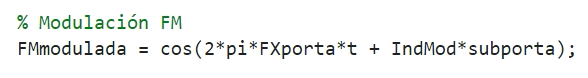
\includegraphics[scale=0.5]{FMmodulada.png}
        \caption{Función que implementa la modulación en FM}
    \end{figure}

\end{frame}










\begin{frame}{Modulación FM}
    \begin{figure}[h]
        \centering
        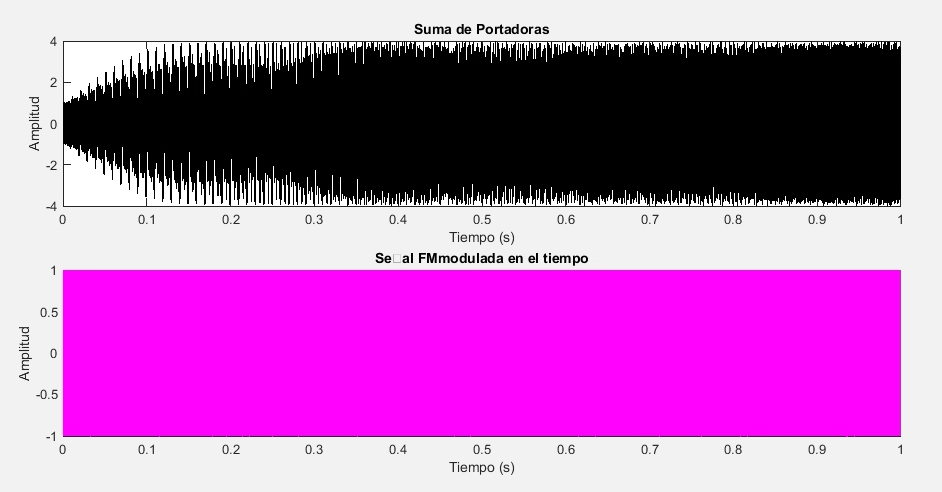
\includegraphics[scale=0.3]{Esp_FM_tiem.png}
        \caption{Señales Modulada en FM en función del Tiempo}
    \end{figure}
\end{frame}

\begin{frame}{Modulación FM}
    \begin{figure}[h]
        \centering
        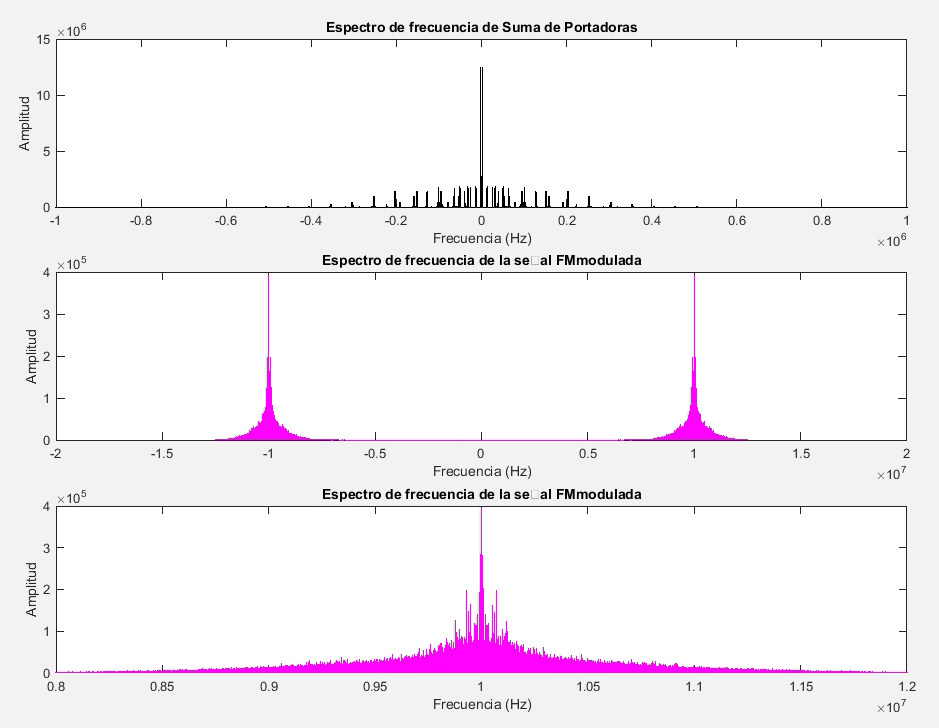
\includegraphics[scale=0.2]{Esp_FM_frec.png}
        \caption{Espetros de las señales generadas por el modulador FM}
    \end{figure}
\end{frame}



\begin{frame}{Modulación FM}
    \begin{figure}[h]
        \centering
        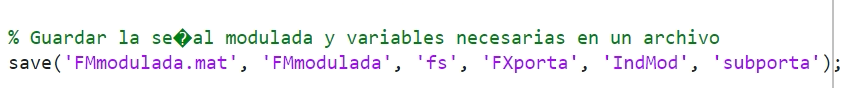
\includegraphics[scale=0.4]{Func_mod.png}
        \caption{Equivalente a transmitir}
    \end{figure}

\end{frame}

\begin{frame}{Modulación FM}
    \begin{figure}[h]
        \centering
        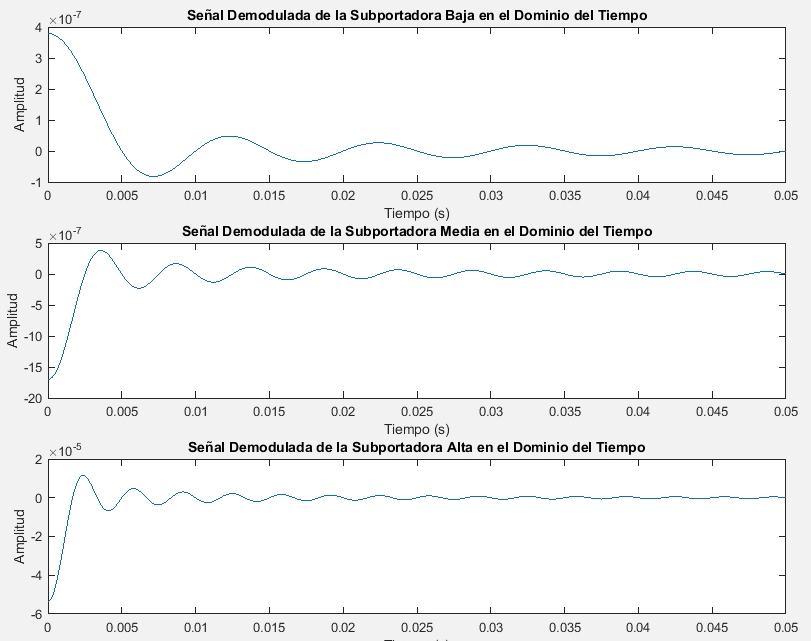
\includegraphics[scale=0.3]{signal_demo.png}
        \caption{Equivalente a transmitir}
    \end{figure}

\end{frame}






\begin{frame}{Modulación FM}
    \begin{figure}[h]
        \centering
        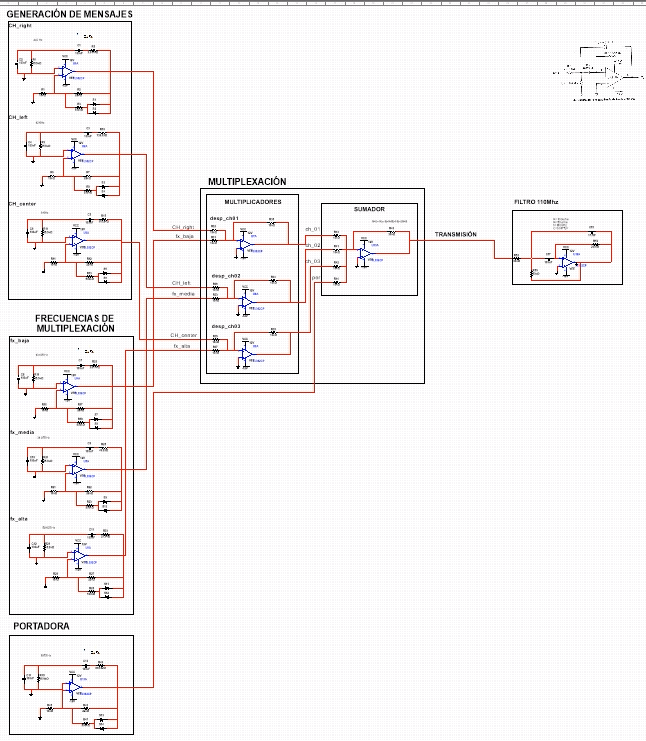
\includegraphics[scale=0.3]{multisim_modul.png}
        \caption{Implementación de modelo discreto del Modulador FM}
    \end{figure}

\end{frame}



\section{Receptor Superheterodino}

\subsection{Parámetros Iniciales y Señal IF}
\begin{frame}{Parámetros Iniciales y Señal IF}
    \begin{itemize}
        \item Carga de la señal modulada desde un archivo.
        \item Creación de un oscilador local de 120.7 MHz.
        \item Mezcla de la señal modulada con el oscilador local para obtener la señal IF.
    \end{itemize}
    \begin{tcolorbox}[colback=yellow!5!white, colframe=yellow!75!black, title=Parámetros Iniciales y Señal IF, fonttitle=\normalsize, fontupper=\normalsize]
\begin{lstlisting}
% Cargar la señal modulada desde el archivo
load('FMmodulada.mat');

% Crear oscilador local de 120.7 MHz para obtener una IF de 10.7 MHz
f_lo = 120.7e6; % Frecuencia del oscilador local
osc_lo = cos(2 * pi * f_lo * t); % Señal del oscilador local

% Mezclar la señal de prueba con el oscilador local para obtener la señal IF
IF_signal = FMmodulada .* osc_lo;
\end{lstlisting}
    \end{tcolorbox}
\end{frame}



\begin{frame}{Parámetros Iniciales y Señal IF}
 
    \begin{figure}[h]
        \centering
        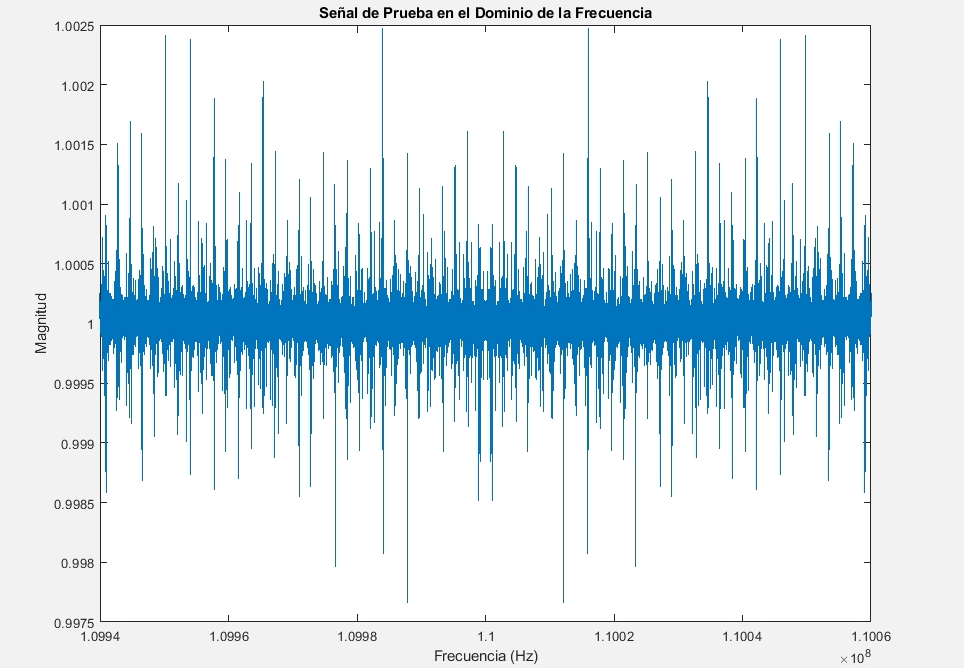
\includegraphics[scale=0.25]{signal_test.png}
        \caption{Espectro de la señal que recibe el Demodulador}
    \end{figure}
    
\end{frame}

\begin{frame}{Parámetros Iniciales y Señal IF}
 
    \begin{figure}[h]
        \centering
        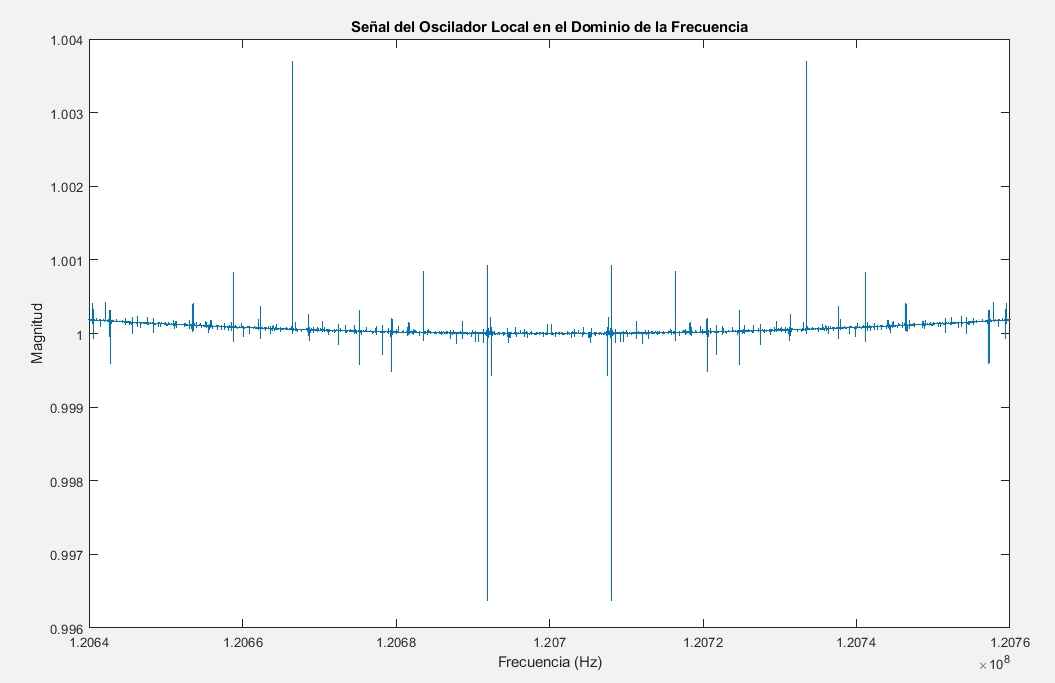
\includegraphics[scale=0.25]{signal_1207.png}
        \caption{Señal Trasladada al del Oscilador Local}
    \end{figure}
    
\end{frame}

\begin{frame}{Parámetros Iniciales y Señal IF}
 
    \begin{figure}[h]
        \centering
        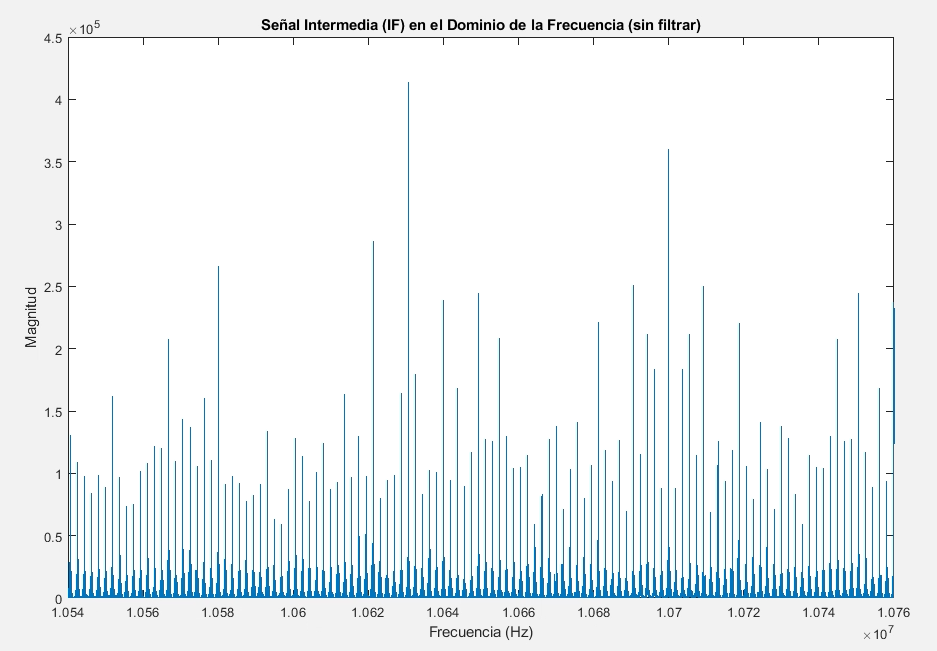
\includegraphics[scale=0.25]{signal_107.png}
        \caption{Señal Trasladada al FI}
    \end{figure}
    
\end{frame}


\subsection{Filtrado de la Señal IF}
\begin{frame}{Filtrado de la Señal IF}
    \begin{itemize}
        \item Aplicación de un filtro en el dominio de la frecuencia para extraer las subportadoras.
    \end{itemize}
    \begin{tcolorbox}[colback=yellow!5!white, colframe=yellow!75!black, title=Filtrado de la Señal IF, fonttitle=\normalsize, fontupper=\normalsize]
\begin{lstlisting}
% Transformar la señal IF al dominio de la frecuencia
IF_signal_freq = fftshift(fft(IF_signal));
f_IF = linspace(-fs/2, fs/2, length(IF_signal_freq)) * fs / length(IF_signal_freq); % Frecuencias para la señal IF

% Aplicar filtro en el dominio de la frecuencia para extraer la componente de 13125 Hz (subportadora)
filtro_pasabanda = (f_IF > (frecuencia_central + fxbaja - 7500)) & (f_IF < (frecuencia_central + fxbaja + 7500));
IF_signal_filtrada_freq = IF_signal_freq .* filtro_pasabanda;
\end{lstlisting}
    \end{tcolorbox}
\end{frame}



\begin{frame}{Parámetros Iniciales y Señal IF}
 
    \begin{figure}[h]
        \centering
        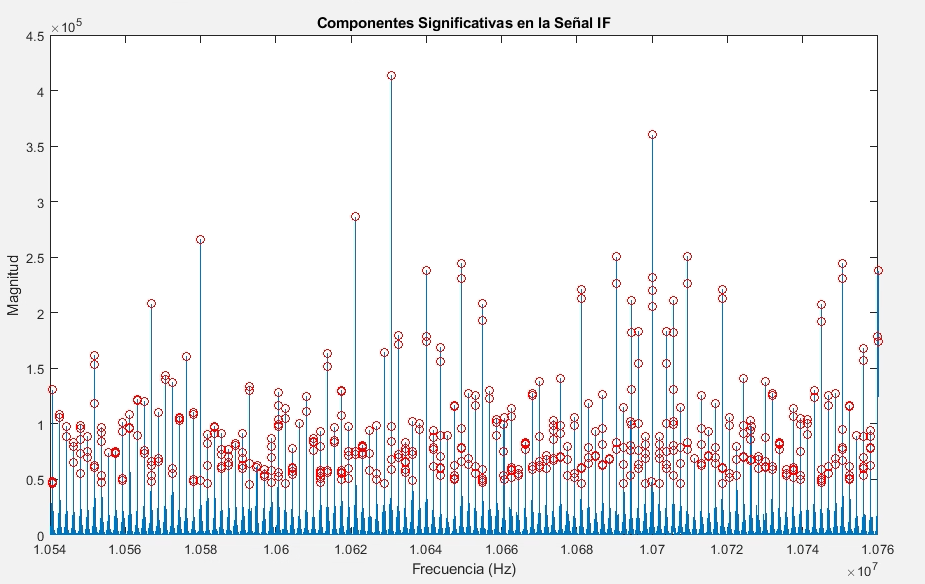
\includegraphics[scale=0.25]{signal_107C.png}
        \caption{Señal de Fi Filtrada}
    \end{figure}
    
\end{frame}

\begin{frame}{Parámetros Iniciales y Señal IF}
 
    \begin{figure}[h]
        \centering
        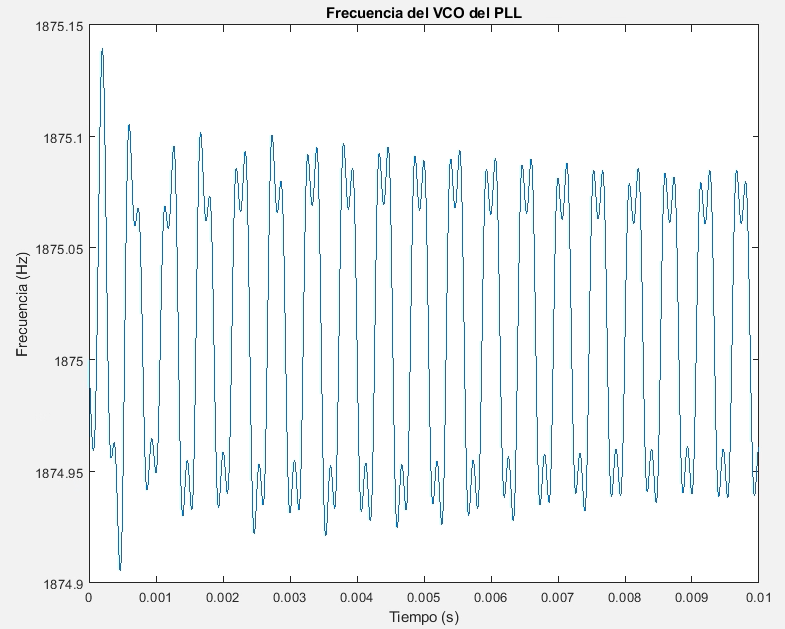
\includegraphics[scale=0.25]{signal_pll.png}
        \caption{Salida del PLL}
    \end{figure}
    
\end{frame}

























\section{Demodulador FM}

\subsection{Demodulación de Subportadoras}
\begin{frame}{Demodulación de Subportadoras}
    \begin{itemize}
        \item Demodulación de las subportadoras extraídas de la señal IF para recuperar las señales de audio originales.
    \end{itemize}
    \begin{tcolorbox}[colback=yellow!5!white, colframe=yellow!75!black, title=Demodulación de Subportadoras, fonttitle=\normalsize, fontupper=\normalsize]
\begin{lstlisting}
% Transformar la señal filtrada de vuelta al dominio del tiempo
IF_signal_filtrada = ifft(ifftshift(IF_signal_filtrada_freq));

% Demodular la subportadora para extraer la señal de prueba de 10 Hz
demodulated_signal = IF_signal_filtrada .* cos(2 * pi * fxbaja * t);
\end{lstlisting}
    \end{tcolorbox}
\end{frame}





\begin{frame}{Parámetros Iniciales y Señal IF}
 
    \begin{figure}[h]
        \centering
        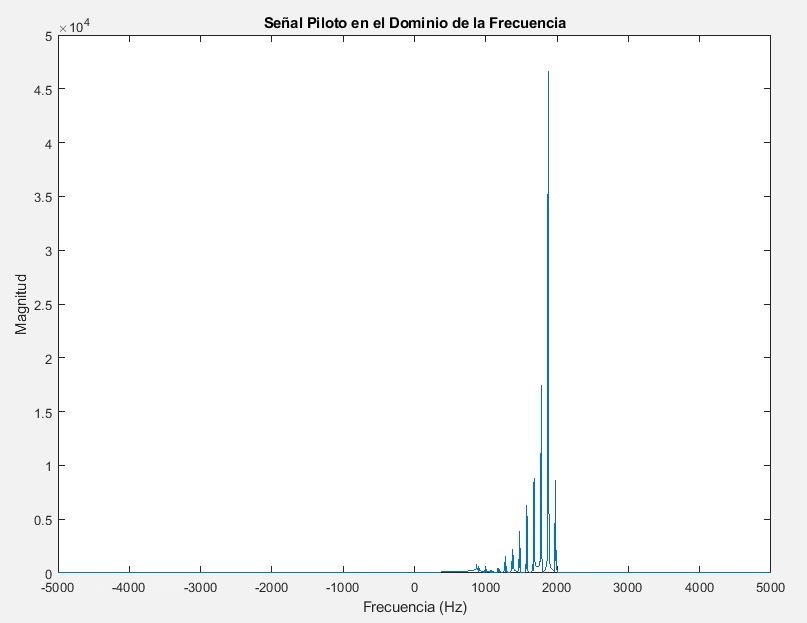
\includegraphics[scale=0.25]{signal_piloto.png}
        \caption{Espectro de la señal Piloto luego de filtrarla}
    \end{figure}
    
\end{frame}


\subsection{Aplicación de Deénfasis}
\begin{frame}{Aplicación de Deénfasis}
    \begin{itemize}
        \item Aplicación de un filtro de deénfasis para compensar el preénfasis aplicado en el transmisor.
        \item Ajuste de la ganancia de las señales demoduladas.
    \end{itemize}
    \begin{tcolorbox}[colback=yellow!5!white, colframe=yellow!75!black, title=Aplicación de Deénfasis y Ajuste de Ganancia, fonttitle=\normalsize, fontupper=\normalsize]
\begin{lstlisting}
% Aplicar filtro en el dominio de la frecuencia para eliminar la componente de alta frecuencia
filtro_pasabaja = (abs(f_demodulated_signal) < Right); % Frecuencia de corte ajustada a la frecuencia de Right
demodulated_signal_freq_filtrada = demodulated_signal_freq .* filtro_pasabaja;

% Transformar la señal filtrada de vuelta al dominio del tiempo
demodulated_signal_filtrada = ifft(ifftshift(demodulated_signal_freq_filtrada));

% Ganancia adicional para la señal demodulada
ganancia = max(abs(fxRight)) / max(abs(demodulated_signal_filtrada));
demodulated_signal_filtrada = demodulated_signal_filtrada * ganancia;
\end{lstlisting}
    \end{tcolorbox}
\end{frame}


\subsection{Demodulación de Cada Señal}



\begin{frame}{Demodulación de Cada Señal}
    \begin{itemize}
        \item Demodulación de las señales utilizando la frecuencia intermedia, recuperando así las tres señales de audio independientes originales.
    \end{itemize}
    \begin{tcolorbox}[colback=yellow!5!white, colframe=yellow!75!black, title=Demodulación de Cada Señal, fonttitle=\normalsize, fontupper=\normalsize]
\begin{lstlisting}
% Demodulación de las señales montadas en las subportadoras fxbajadem, fxmediadem, fxaltadem
% Demodulación de fxbajadem
filtro_pasabanda_baja = (f_IF > (frecuencia_central + fxbajadem - 7500)) & (f_IF < (frecuencia_central + fxbajadem + 7500));
IF_signal_baja_filtrada_freq = IF_signal_freq .* filtro_pasabanda_baja;
IF_signal_baja_filtrada = ifft(ifftshift(IF_signal_baja_filtrada_freq));
demodulated_signal_baja = IF_signal_baja_filtrada .* cos(2 * pi * fxbajadem * t);

% Demodulación de fxmediadem
filtro_pasabanda_media = (f_IF > (frecuencia_central + fxmediadem - 7500)) & (f_IF < (frecuencia_central + fxmediadem + 7500));
IF_signal_media_filtrada_freq = IF_signal_freq .* filtro_pasabanda_media;
IF_signal_media_filtrada = ifft(ifftshift(IF_signal_media_filtrada_freq));
demodulated_signal_media = IF_signal_media_filtrada .* cos(2 * pi * fxmediadem * t);

% Demodulación de fxaltadem
filtro_pasabanda_alta = (f_IF > (frecuencia_central + fxaltadem - 7500)) & (f_IF < (frecuencia_central + fxaltadem + 7500));
IF_signal_alta_filtrada_freq = IF_signal_freq .* filtro_pasabanda_alta;
IF_signal_alta_filtrada = ifft(ifftshift(IF_signal_alta_filtrada_freq));
demodulated_signal_alta = IF_signal_alta_filtrada .* cos(2 * pi * fxaltadem * t);
\end{lstlisting}
    \end{tcolorbox}
\end{frame}

\begin{frame}{Demodulación discreta}

    \begin{figure}[h]
        \centering
        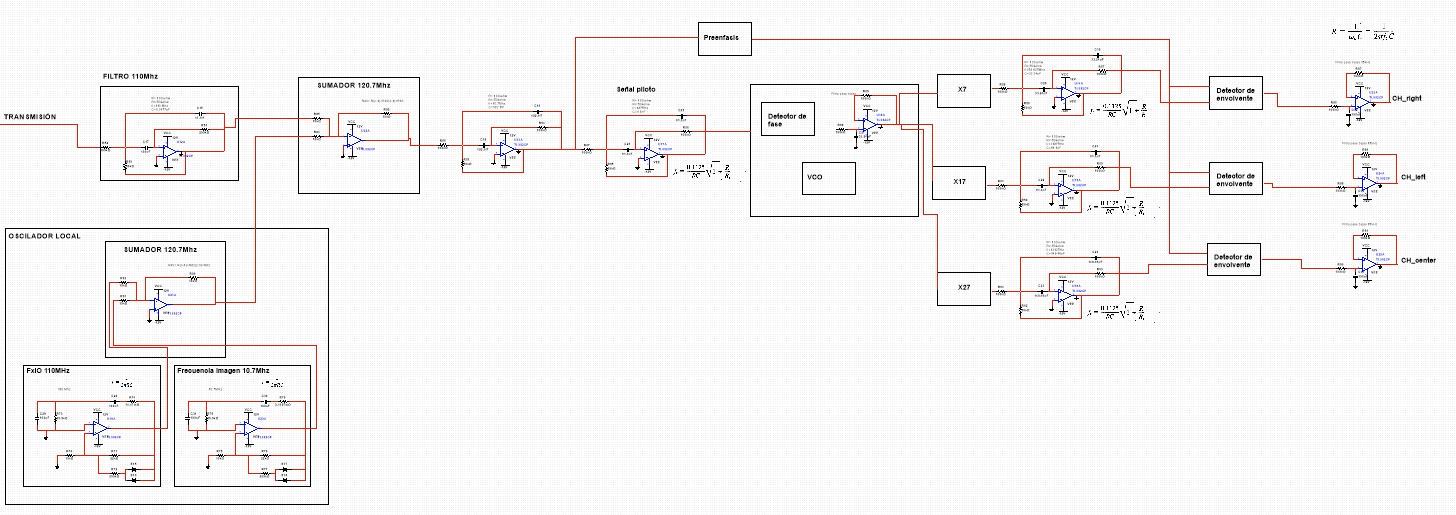
\includegraphics[scale=0.25]{mulsis_demod.png}
        \caption{Espectro de la señal Piloto luego de filtrarla}
    \end{figure}

\end{frame}


\section{Conclusiones}
\begin{frame}{Conclusiones}
    \begin{itemize}
        \item La implementación del modulador y demodulador FM en MATLAB/Octave fue exitosa.
        \item La transmisión y recuperación de las señales de audio multiplexadas se realizó de manera eficiente.
        \item La estructura modular del código facilita futuras modificaciones y adaptaciones del sistema.
    \end{itemize}
\end{frame}

\section{Mejoras}
\begin{frame}{Mejoras}
    \begin{itemize}
        \item Considerar la implementación de técnicas adicionales para reducir el ruido en la señal transmitida.
        \item Optimizar el código para mejorar el rendimiento y reducir el tiempo de procesamiento.
        \item Investigar y proponer simulaciones adicionales para validar el desempeño del sistema en diferentes condiciones.
    \end{itemize}
\end{frame}

\end{document}
